\documentclass[conference]{IEEEtran}
\IEEEoverridecommandlockouts
% The preceding line is only needed to identify funding in the first footnote. If that is unneeded, please comment it out.
\usepackage{cite}
\usepackage{amsmath,amssymb,amsfonts}
\usepackage{algorithmic}
\usepackage{graphicx}
\usepackage{textcomp}
\usepackage{xcolor}
\usepackage{float}

\def\BibTeX{{\rm B\kern-.05em{\sc i\kern-.025em b}\kern-.08em
    T\kern-.1667em\lower.7ex\hbox{E}\kern-.125emX}}
\begin{document}

\title{Detection of heart anomalies by use of adaptive LMS filters in ECG signals*\\
{\footnotesize \textsuperscript{*}Note: Sub-titles are not captured in Xplore and
should not be used}
}

\author{\IEEEauthorblockN{1\textsuperscript{st} Tom\'as Agust\'in Gonz\'alez Orlando}
\IEEEauthorblockA{\textit{dept. name of organization (of Aff.)} \\
\textit{name of organization (of Aff.)}\\
Buenos Aires, Argentina\\
togonzalez@itba.edu.ar}
\and
\IEEEauthorblockN{2\textsuperscript{nd} Ariel Santiago Nowik}
\IEEEauthorblockA{\textit{dept. name of organization (of Aff.)} \\
\textit{name of organization (of Aff.)}\\
Buenos Aires, Argentina\\
anowik@itba.edu.ar}
}

\maketitle

\begin{abstract}
An implementation of a heart anomaly detector for non-paced rhythms using different adaptive filter structures is proposed.\par
The detection algorithm uses an Adaptive Recursive Filter (ARF), for which the impulse input is previously determined via a peak localization and time shift estimation algorithm. \par
The detection of each anomaly by itself is product of the direct observation of the magnitude of the ARF output.
The design and testing of the detector was based on the MIT-BIH Arrhythmia Database with almost none false-negative and few false-positive results.
\end{abstract}

\begin{IEEEkeywords}
ECG analysis, heart anomaly detection, Adaptive Filtering, LMS filters
\end{IEEEkeywords}


\section{Introduction}


\subsection{Electrocardiogram signals}

An Electrocardiogram (ECG) signal is a non invasive recording (electrodes are placed on the patient's skin) of the electrical activity of a heart. There are several places where the signals may be recorded, and usually as many as ten electrodes are used to perform an ECG, where the polarization and repolarization of the heart muscles are recorded. \par
An ECG portrays an incredibly large amount of information from the patient, such as the rate and rhythm of heartbeats, the size and position of the heart chambers, the presence of any damage to the heart's muscle cells or conduction system, the effects of heart drugs, and the function of implanted pacemakers.\par
These polarization cycles form the main three components of a heart signal, which are listed as follows:
\begin{itemize}
\item \underline{P-wave} : Depolarization of the atria. This component is frequently the one with the lowest amplitude.
\item \underline{QRS complex}: Depolarization of the ventricles. In the QRS complex a peak of high frequency and the highest amplitude is detected. 
\item \underline{T-wave}: Repolarization of the ventricles.
\end{itemize} 

\begin{figure}[htbp]
\centerline{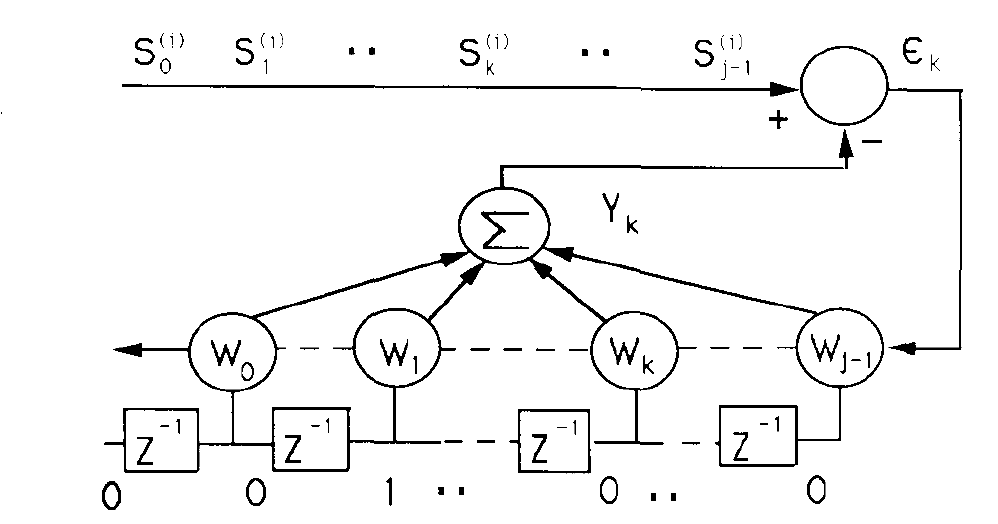
\includegraphics[scale=0.7]{ARF_diagram.png}}
\caption{Basic diagram of an ARF}
\label{fig}
\end{figure}

These components were enumerated in their usual order of appearance. However, some patients with heart abnormalities exhibit a P-wave that superposes over the QRS complex, so the techniques developed below should take into account this factor when analysing the ECG signal even with no previous knowledge of the abnormality. Adaptive filters have been proven efficient in such cases. \par

\subsection{Adaptive Recursive Filters}

An Adaptive Recursive Filter (ARF) is an adaptive filter whose coefficients change so that when it is adapted, its impulse response converges to a single pseudo-period of an ideally periodic signal. The ARF is therefore applied to signals that are known to have periodic behaviour with considerably small changes through time in both its pseudo-periods and its fundamental period.\par
The signal in question may be then considered to be stationary between time intervals of a given length.\par
A diagram of the ARF, taken from \cite{b1} is shown below:

\begin{figure}[H]
\centerline{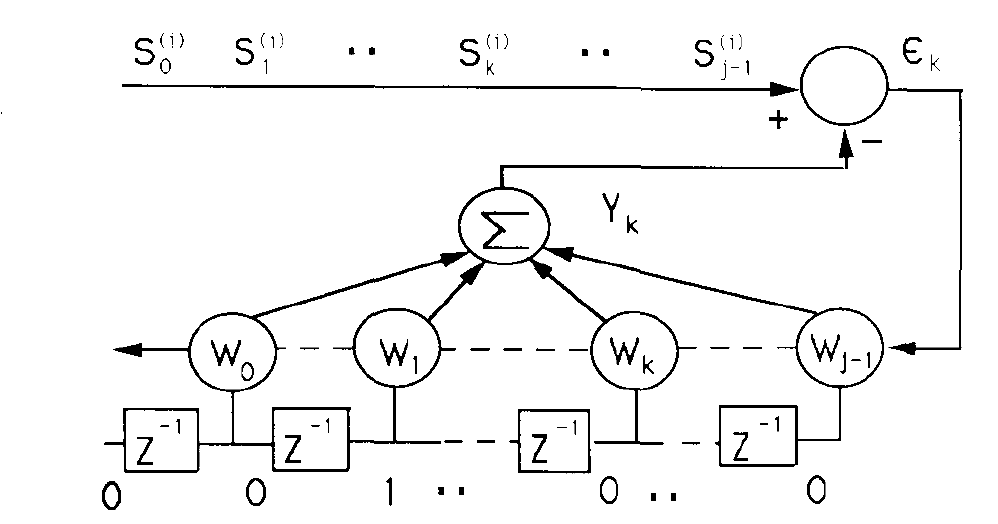
\includegraphics[scale=0.7]{ARF_diagram.png}}
\caption{Basic diagram of an ARF}
\label{fig}
\end{figure}


\section{LMS prediction}

The first approach taken was the implementation of an adaptive predictor based on the following diagram:
\begin{figure}[H]
\centerline{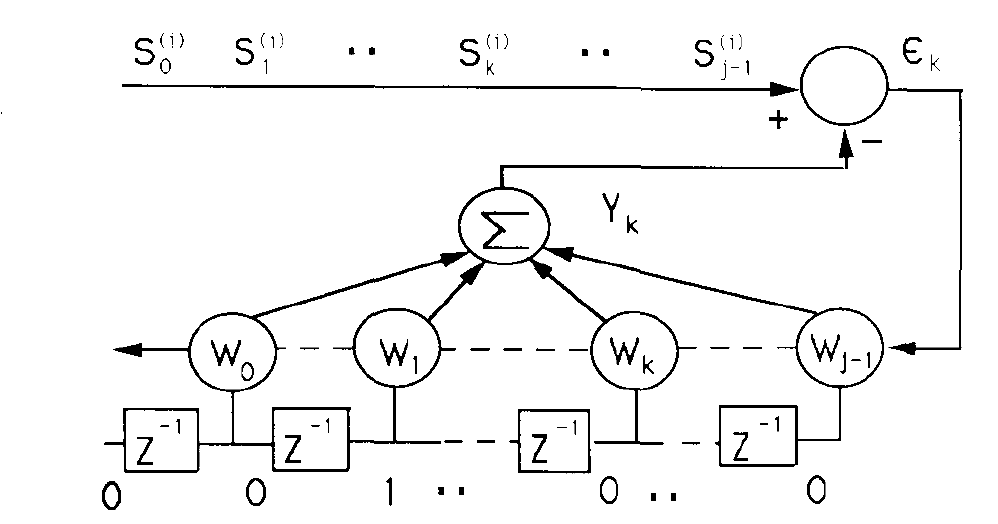
\includegraphics[scale=0.7]{ARF_diagram.png}}
\caption{Basic diagram of an ARF}
\label{fig}
\end{figure}

The implementation achieved its desired purpose of predicting the signal, as shown in the following figure:

\begin{figure}[H]
\centerline{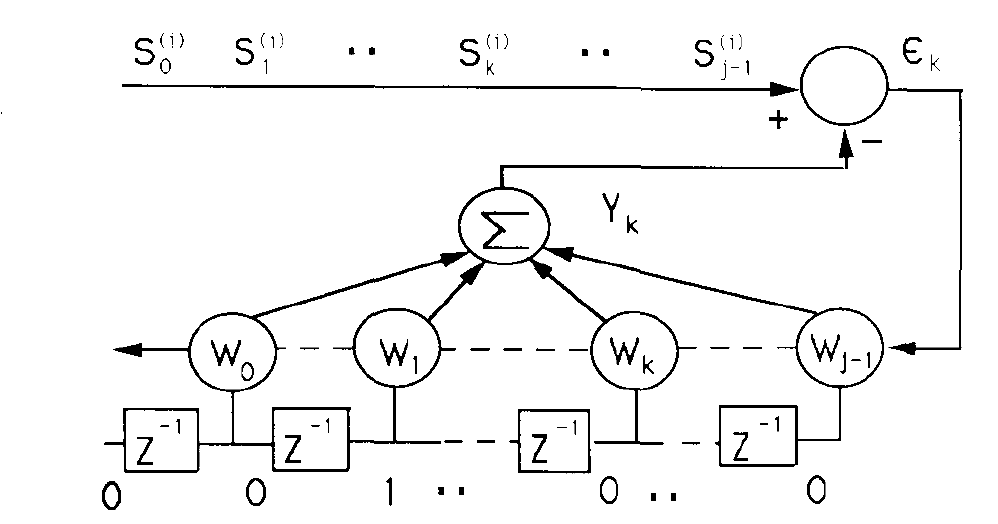
\includegraphics[scale=0.7]{ARF_diagram.png}}
\caption{Signal 202 of the MIT-BIH Arrhythmia Database, minute , and the predictor's response.}
\label{fig}
\end{figure}

The magnitude of the error signal was afterwards processed in order to get its peaks, which where considered anomalies when its amplitude exceeded a designated value. This method of anomaly detection did not manage to achieve acceptable results as the predictor error tends to raise when the ECG signal has high frequency changes, and so the the peaks of the QRS complex were also taken as anomalies. \par
Although this problem disqualified the method, if the QRS complex is detected via a previous analysis of the signal, discarding the false positives that appear with its peaks may be a path to be followed in future investigations.\par

\section{Detection}

The detection of each anomaly consists of applying the detection algorithm to the entire ECG signal or a portion of it. The steps of this algorithm are in line with the arrythmia detection method stated by \cite{b1}:

\begin{enumerate}
\item Find the peaks of each QRS complex.
\item Generate an impulse signal in which each impulse coincides with the beggining of the QRS complex.  
\item Feed the ARF with both the new impulse signal and the ECG. 
\item Get the error signal of the ARF after processing the inputs.
\item Identify the peaks of the absolute error signal and select those points in which these peaks may signify an anomaly.
\end{enumerate}

Choosing to generate an impulse at the start of the QRS complex and not at the start of the P-wave is the solution for the possibility of an abnormality in the P-wave that may provoke it to overlap with other components of the signal. The ARF will make its impulse response copy by default the QRS complex and the T-wave, and in such case that no overlapping ocurrs, the P-wave will also be shown in the impulse response of the filter.

\subsection{Detection of the QRS complex}

The localization of the QRS complex is based on the detection of high amplitude peaks. This may be done by assuming signal stationarity for some interval of time. Fifteen pseudo-periods of the signal has been proven an effective amount of time. The period has been estimated with the a priori knowledge of an ECG: The period of a heart signal is of approximately 1 beat per second. Taking this into account and the fact that the sample rate of the MIT-BIH Database is 360 Hz, a number of 350 samples was the estimated length of a heart beat. \par
After defining the stationary interval, the signal is then converted to its energy signal by simply squaring each value. Converting the signal to its energy signal for peak detection has two advantages:

\begin{enumerate}
\item All values of the energy signal will be non negative.
\item Greater values will be weigthed as more important and significative than smaller values as pondered by the square function.
\end{enumerate}

A peak will be detected each time a sample of the energy signal has a value that is at least 0.55 times the maximum value of the interval.

\subsection{Generation of the impulse signal}

As each peak of the QRS complex corresponds to the R component of the signal, a time shift should be applied so that the generated impulse signal will have its impulse assigned to the beginning of the QRS complex. This time shift should also be estimated in a proportion of the estimated pseudo-period time.

\section{Accuracy of the method}
Before you begin to format your paper, first write and save the content as a 
separate text file. Complete all content and organizational editing before 
formatting. Please note sections \ref{AA}--\ref{SCM} below for more information on 
proofreading, spelling and grammar.

Keep your text and graphic files separate until after the text has been 
formatted and styled. Do not number text heads---{\LaTeX} will do that 
for you.


\subsection{Equations}
Number equations consecutively. To make your 
equations more compact, you may use the solidus (~/~), the exp function, or 
appropriate exponents. Italicize Roman symbols for quantities and variables, 
but not Greek symbols. Use a long dash rather than a hyphen for a minus 
sign. Punctuate equations with commas or periods when they are part of a 
sentence, as in:
\begin{equation}
a+b=\gamma\label{eq}
\end{equation}

Be sure that the 
symbols in your equation have been defined before or immediately following 
the equation. Use ``\eqref{eq}'', not ``Eq.~\eqref{eq}'' or ``equation \eqref{eq}'', except at 
the beginning of a sentence: ``Equation \eqref{eq} is . . .''

\subsection{\LaTeX-Specific Advice}

Please use ``soft'' (e.g., \verb|\eqref{Eq}|) cross references instead
of ``hard'' references (e.g., \verb|(1)|). That will make it possible
to combine sections, add equations, or change the order of figures or
citations without having to go through the file line by line.

Please don't use the \verb|{eqnarray}| equation environment. Use
\verb|{align}| or \verb|{IEEEeqnarray}| instead. The \verb|{eqnarray}|
environment leaves unsightly spaces around relation symbols.

Please note that the \verb|{subequations}| environment in {\LaTeX}
will increment the main equation counter even when there are no
equation numbers displayed. If you forget that, you might write an
article in which the equation numbers skip from (17) to (20), causing
the copy editors to wonder if you've discovered a new method of
counting.

{\BibTeX} does not work by magic. It doesn't get the bibliographic
data from thin air but from .bib files. If you use {\BibTeX} to produce a
bibliography you must send the .bib files. 

{\LaTeX} can't read your mind. If you assign the same label to a
subsubsection and a table, you might find that Table I has been cross
referenced as Table IV-B3. 

{\LaTeX} does not have precognitive abilities. If you put a
\verb|\label| command before the command that updates the counter it's
supposed to be using, the label will pick up the last counter to be
cross referenced instead. In particular, a \verb|\label| command
should not go before the caption of a figure or a table.

Do not use \verb|\nonumber| inside the \verb|{array}| environment. It
will not stop equation numbers inside \verb|{array}| (there won't be
any anyway) and it might stop a wanted equation number in the
surrounding equation.

\subsection{Some Common Mistakes}\label{SCM}
\begin{itemize}
\item The word ``data'' is plural, not singular.
\item The subscript for the permeability of vacuum $\mu_{0}$, and other common scientific constants, is zero with subscript formatting, not a lowercase letter ``o''.
\item In American English, commas, semicolons, periods, question and exclamation marks are located within quotation marks only when a complete thought or name is cited, such as a title or full quotation. When quotation marks are used, instead of a bold or italic typeface, to highlight a word or phrase, punctuation should appear outside of the quotation marks. A parenthetical phrase or statement at the end of a sentence is punctuated outside of the closing parenthesis (like this). (A parenthetical sentence is punctuated within the parentheses.)
\item A graph within a graph is an ``inset'', not an ``insert''. The word alternatively is preferred to the word ``alternately'' (unless you really mean something that alternates).
\item Do not use the word ``essentially'' to mean ``approximately'' or ``effectively''.
\item In your paper title, if the words ``that uses'' can accurately replace the word ``using'', capitalize the ``u''; if not, keep using lower-cased.
\item Be aware of the different meanings of the homophones ``affect'' and ``effect'', ``complement'' and ``compliment'', ``discreet'' and ``discrete'', ``principal'' and ``principle''.
\item Do not confuse ``imply'' and ``infer''.
\item The prefix ``non'' is not a word; it should be joined to the word it modifies, usually without a hyphen.
\item There is no period after the ``et'' in the Latin abbreviation ``et al.''.
\item The abbreviation ``i.e.'' means ``that is'', and the abbreviation ``e.g.'' means ``for example''.
\end{itemize}
An excellent style manual for science writers is \cite{b7}.

\subsection{Authors and Affiliations}
\textbf{The class file is designed for, but not limited to, six authors.} A 
minimum of one author is required for all conference articles. Author names 
should be listed starting from left to right and then moving down to the 
next line. This is the author sequence that will be used in future citations 
and by indexing services. Names should not be listed in columns nor group by 
affiliation. Please keep your affiliations as succinct as possible (for 
example, do not differentiate among departments of the same organization).

\subsection{Identify the Headings}
Headings, or heads, are organizational devices that guide the reader through 
your paper. There are two types: component heads and text heads.

Component heads identify the different components of your paper and are not 
topically subordinate to each other. Examples include Acknowledgments and 
References and, for these, the correct style to use is ``Heading 5''. Use 
``figure caption'' for your Figure captions, and ``table head'' for your 
table title. Run-in heads, such as ``Abstract'', will require you to apply a 
style (in this case, italic) in addition to the style provided by the drop 
down menu to differentiate the head from the text.

Text heads organize the topics on a relational, hierarchical basis. For 
example, the paper title is the primary text head because all subsequent 
material relates and elaborates on this one topic. If there are two or more 
sub-topics, the next level head (uppercase Roman numerals) should be used 
and, conversely, if there are not at least two sub-topics, then no subheads 
should be introduced.

\subsection{Figures and Tables}
\paragraph{Positioning Figures and Tables} Place figures and tables at the top and 
bottom of columns. Avoid placing them in the middle of columns. Large 
figures and tables may span across both columns. Figure captions should be 
below the figures; table heads should appear above the tables. Insert 
figures and tables after they are cited in the text. Use the abbreviation 
``Fig.~\ref{fig}'', even at the beginning of a sentence.

\begin{table}[htbp]
\caption{Table Type Styles}
\begin{center}
\begin{tabular}{|c|c|c|c|}
\hline
\textbf{Table}&\multicolumn{3}{|c|}{\textbf{Table Column Head}} \\
\cline{2-4} 
\textbf{Head} & \textbf{\textit{Table column subhead}}& \textbf{\textit{Subhead}}& \textbf{\textit{Subhead}} \\
\hline
copy& More table copy$^{\mathrm{a}}$& &  \\
\hline
\multicolumn{4}{l}{$^{\mathrm{a}}$Sample of a Table footnote.}
\end{tabular}
\label{tab1}
\end{center}
\end{table}

\begin{figure}[htbp]
\centerline{
\includegraphics{fig1.png}}
\caption{Example of a figure caption.}
\label{fig}
\end{figure}

Figure Labels: Use 8 point Times New Roman for Figure labels. Use words 
rather than symbols or abbreviations when writing Figure axis labels to 
avoid confusing the reader. As an example, write the quantity 
``Magnetization'', or ``Magnetization, M'', not just ``M''. If including 
units in the label, present them within parentheses. Do not label axes only 
with units. In the example, write ``Magnetization (A/m)'' or ``Magnetization 
\{A[m(1)]\}'', not just ``A/m''. Do not label axes with a ratio of 
quantities and units. For example, write ``Temperature (K)'', not 
``Temperature/K''.

\section*{Acknowledgment}

The preferred spelling of the word ``acknowledgment'' in America is without 
an ``e'' after the ``g''. Avoid the stilted expression ``one of us (R. B. 
G.) thanks $\ldots$''. Instead, try ``R. B. G. thanks$\ldots$''. Put sponsor 
acknowledgments in the unnumbered footnote on the first page.

\section*{References}

Please number citations consecutively within brackets \cite{b1}. The 
sentence punctuation follows the bracket \cite{b2}. Refer simply to the reference 
number, as in \cite{b3}---do not use ``Ref. \cite{b3}'' or ``reference \cite{b3}'' except at 
the beginning of a sentence: ``Reference \cite{b3} was the first $\ldots$''

Number footnotes separately in superscripts. Place the actual footnote at 
the bottom of the column in which it was cited. Do not put footnotes in the 
abstract or reference list. Use letters for table footnotes.

Unless there are six authors or more give all authors' names; do not use 
``et al.''. Papers that have not been published, even if they have been 
submitted for publication, should be cited as ``unpublished'' \cite{b4}. Papers 
that have been accepted for publication should be cited as ``in press'' \cite{b5}. 
Capitalize only the first word in a paper title, except for proper nouns and 
element symbols.

For papers published in translation journals, please give the English 
citation first, followed by the original foreign-language citation \cite{b6}.

\begin{thebibliography}{00}
\bibitem{b1} Nitish V. Thakor and Yi-Sheng Zhu, ``Applications of Adaptive Filtering to ECG Analysis :
Noise Cancellation and Arrhythmia Detection'', IEEE Transactions On Biomedical Engineering. Vol. 18. No 8. August 1991.
\end{thebibliography}
\vspace{12pt}
\color{red}
IEEE conference templates contain guidance text for composing and formatting conference papers. Please ensure that all template text is removed from your conference paper prior to submission to the conference. Failure to remove the template text from your paper may result in your paper not being published.

\end{document}
